% !TEX root = ../thesis.tex

\chapter{Pravdepodobnostná analýza kvantových obvodov}
\label{pravAnalL}

V predošlých kapitolách bola vysvetlená problematika kvantových obvodov.
Našou úlohou je merať stavy kvantových bitov v rôznych časových okamihoch.
Je možné zostrojiť nekonečné množstvo rôznych kvantových obvodov,
a preto v tejto kapitole priblížime spôsob tohto merania.
Vo všeobecnosti môžme rozdeliť kvantové obvody na dva druhy, v ktorých 
meranie má iný charakter. Sú to obvody s nepreviazanými bitmi a obvody s 
previazanými kvantovými bitmi.

\section{Analýza nepreviazaných stavov}

\begin{figure} 
	\centering 
	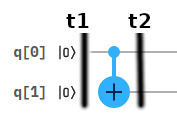
\includegraphics[width=.4\textwidth]{figures/simpleCircuit2.png} 
	\caption{Jednotduchý kvantový obvod (namodelovaný v IBM Quantum Experience)}
    \label{obvod}
\end{figure}

Na obrázku \ref{obvod} je vygenerovaný jednoduchý kvantový obvod pomocou
nástroja IBM Quantum Experience. Označili sme dva časové úseky 
\(t_1\) a \(t_2\). V tomto obvode sú dva kvantové bity, ktoré prechádzajú 
hradlom CNOT. Pre 
zachovanie notácie budeme ďalej označovať tieto bity ako 
\(\psi_0\) a \(\psi_1\). Z kvantového obvodu je zrejmé, že v čase \(t_1\) 
sú oba kvantové bity v stave
\(\ket{0}\), to ale nebudeme brať v úvahu. Zaujíma nás pravdepodobnosť 
namerania stavov \(\ket{00}, \ket{01}, \ket{10}\) a \(\ket{11}\).

Vieme, že platí \(\ket{\psi_0} = \binom{\alpha_0}{\beta_0}\) a  
\(\ket{\psi_1} = \binom{\alpha_1}{\beta_1}\), a teda pre celkový stav \(\psi\) 
platí 
\[
\ket{\psi} = \ket{\psi_0} \otimes \ket{\psi_1} = \binom{\alpha_0}{\beta_0}
\otimes \binom{\alpha_1}{\beta_1} = 
\begin{pmatrix}
    \alpha_0\alpha_1 \\
    \alpha_0\beta_1 \\
    \beta_0\alpha_1 \\
    \beta_0\beta_1
\end{pmatrix}
\]
Z toho vyplíva, že celkový stav \(\ket{\psi}\) v čase \(t_1\) nadobúda 
hodnoty
\begin{itemize}
    \item[] \(\ket{00}\) s pravdepodobnosťou \(\Vert \alpha_0\alpha_1 \Vert^2\)
    \item[] \(\ket{01}\) s pravdepodobnosťou \(\Vert \alpha_0\beta_1 \Vert^2\)
    \item[] \(\ket{10}\) s pravdepodobnosťou \(\Vert \beta_0\alpha_1 \Vert^2\)
    \item[] \(\ket{11}\) s pravdepodobnosťou \(\Vert \beta_0\beta_1 \Vert^2\)
\end{itemize}

Toto tvrdenie platí, pretože platí 
\(\ket{\psi_0} = \alpha_0\ket{0} + \beta_0\ket{1}\), čiže 
\(|\alpha_0|^2 + |\beta_0|^2 = 1\), z čoho vyplíva, že 
\begin{itemize}
    \item[] \(\ket{\psi_0}\) nadobúda hodontu 0 s 
pravdepodobnosťou \(|\alpha_0|^2\) a 
    \item[] \(\ket{\psi_0}\) nadobúda hodontu 1 s 
pravdepodobnosťou \(|\beta_0|^2\).
\end{itemize}
Obdobne to platí aj pre \(\ket{\psi_1}\). K rovnakému záveru sa dopracujeme
aj pomocou 
\[\ket{\psi} = \ket{\psi_0} \otimes \ket{\psi_1} = 
(\alpha_0\ket{0} + \beta_0\ket{1}) \otimes  (\alpha_1\ket{0} + \beta_1\ket{1}) =
\]
\[
\alpha_0\alpha_1 (\ket{0} \otimes \ket{0}) +  
\alpha_0\beta_1 (\ket{0} \otimes \ket{1}) + 
\beta_0\alpha_1 (\ket{1} \otimes \ket{0}) + 
\beta_0\beta_1 (\ket{1} \otimes \ket{1}) 
\]
, čo by sme mohli vyjadriť aj iným zápisom ako 
\(
\alpha_{00}\ket{00} + \alpha_{01}\ket{01} + 
\alpha_{10}\ket{10} + \alpha_{11}\ket{11}
\), pričom súčet noriem musí byť rovný 1.
\[
|\alpha_{00}|^2 + |\alpha_{01}|^2 + |\alpha_{10}|^2 + |\alpha_{11}|^2 = 1\]

\section{Analýza previazaných stavov}

Pri meraní stavov v čase \(t_2\), už nemožno dostať výsledný stav \(\psi\)
priamim využitím tenzorového súčinu. Pri prechode hradom CNOT môžu nastať
dve situácie:
\begin{enumerate}
    \item Kvantový bit \(\psi_0\), ktorý je kontrólnym bitom, je v stave 
\(\ket{1}\) a teda nastane preklopenie bitu \(\psi_1\), čo je cieľoým bitom,
pomocou hradla X,
    \item Kvantový bit \(\psi_0\) nie je v stave \(\ket{1}\) a teda bit 
\(\psi_1\) pokračuje bez zmeny.
\end{enumerate}

Z toho je jasné, že v kažom prípade sa stav \(\ket{\psi_0}\) nemení no
stav \(\ket{\psi_1}\) nadobúda hodnotu:
\begin{itemize}
    \item \(\ket{\psi_1}\) s pravdepodobnosťou \(|\alpha_0|^2\),
    \item \(X\ket{\psi_1}\) s pravdepodobnosťou \(|\beta_0|^2\).
\end{itemize}
Berme v úvahu to, že v príklade sme využili hradlo CNOT. Pri pohľade na 
viacbitový systém s využitím haradla CCNOT, kde máme viacero kontrólnych bitov,
zisťujeme, že odvodzovanie je netriviálne a tento problém je nutné riešiť
pomocou pravdepodobnostného rozhodovacieho stromu (o tom v ďalších kapitolách).
